\documentclass[11pt,ngerman,a4paper]{article}
\usepackage{geometry}
\geometry{a4paper,left=30mm,right=25mm, top=3cm, bottom=2cm} 
\usepackage[utf8]{inputenc}
\usepackage{amsmath}
\usepackage{amsfonts}
\usepackage{amssymb}
\usepackage{graphicx}
\usepackage{hyperref}
\usepackage{color}
\usepackage{colortbl}
\usepackage{subfigure}
\usepackage{epstopdf}
\usepackage{multirow}
\usepackage{listings}
\usepackage{setspace}
\usepackage{pdfpages}
\usepackage{trfsigns}


\usepackage[automark,headsepline, footsepline]{scrpage2}

%defines
\def\TReg{\textsuperscript{\textregistered}}
\def\trans{^\mathrm{T}}
\newcommand{\mb}{\mathbf}
\def\*{\cdot}

% no indent but a free line after paragraphs
\setlength{\parindent}{0pt}
\setlength{\parskip}{1.5ex}

\setcounter{secnumdepth}{3}  %Nummerierung vertiefen *
\renewcommand*\thesubsubsection{\alph{subsection} \arabic{subsubsection}.)}
\renewcommand*\thesubsection{\alph{subsection})}
\renewcommand*\thesection{2.\arabic{section}}

% styling and meta-infos
\hypersetup
{
colorlinks=true,
linkcolor=blue,
citecolor=blue,
urlcolor=blue
}


\definecolor{dkgreen}{rgb}{0,0.6,0}
\definecolor{gray}{rgb}{0.5,0.5,0.5}
\definecolor{mauve}{rgb}{0.58,0,0.82}
 
\lstset{ %
  language=C,                % the language of the code
  basicstyle=\footnotesize,           % the size of the fonts that are used for the code
  numbers=left,                   % where to put the line-numbers
  numberstyle=\tiny\color{gray},  % the style that is used for the line-numbers
  stepnumber=2,                   % the step between two line-numbers. If it's 1, each line 
                                  % will be numbered
  numbersep=5pt,                  % how far the line-numbers are from the code
  backgroundcolor=\color{white},      % choose the background color. You must add \usepackage{color}
  showspaces=false,               % show spaces adding particular underscores
  showstringspaces=false,         % underline spaces within strings
  showtabs=false,                 % show tabs within strings adding particular underscores
  frame=single,                   % adds a frame around the code
  rulecolor=\color{black},        % if not set, the frame-color may be changed on line-breaks within not-black text (e.g. commens (green here))
  tabsize=2,                      % sets default tabsize to 2 spaces
  captionpos=b,                   % sets the caption-position to bottom
  breaklines=true,                % sets automatic line breaking
  breakatwhitespace=false,        % sets if automatic breaks should only happen at whitespace
  title=\lstname,                   % show the filename of files included with \lstinputlisting;
                                  % also try caption instead of title
  keywordstyle=\color{blue},          % keyword style
  commentstyle=\color{dkgreen},       % comment style
  stringstyle=\color{mauve},         % string literal style
  escapeinside={\%*}{*)},            % if you want to add a comment within your code
  morekeywords={*,...}               % if you want to add more keywords to the set
}


\pagestyle{scrheadings}

%\ihead[]{} %- linke Kopfzeile
\chead[]{} %- mittlere Kopfzeile
\ohead[]{\pagemark } %- rechte Kopfzeile
\ifoot[]{MSP - 2nd Assignment} %- linke Fußzeile
\cfoot[]{
\includegraphics[height = 12pt]{pics/logo_tu_graz.png}} %- mittlere Fußzeile
\ofoot[]{Ebner, Viehauser} %- rechte Fußzeile


\begin{document}

%
\setcounter{page}{1}
\clearpage
\section{Digital Representation of Continuous-time Systems and Filter Design} 


\clearpage
\section{Performance Characterization of Sampling Systems}

\paragraph{a)}

According to the IEEE Standard the test methods for SINAD, SFDR and SINAD were implemented.
The calculation was quite straightforward and can seen in the matlab file PC\_ADC.m.

\paragraph{b)}

The plots of the different performance measures can be seen in Figure \ref{fig:snrplots}.

You can see that The SFDR stays almost constant over frequency.
The SFDR is calculated by dividing the signal amplitude by the biggest component of noise
and distortion. I observed some kind of distortion in the spectrum (Figure \ref{fig:spectrum}), which
is not in within the first 5 harmonics, but has the highest amplitude. By looking at plots of
different signals, I observed that the amplitude of this distortion stays almost the same over frequency.
Therefore, the SFDR only depends on the signal amplitude and the amplitude of that distortion
and stays almost constant.

The THD decreases very slightly over the frequency. This means that the harmonic distortions are decreasing.

The SINAD decreases over the frequency. Because the Signal stays the same and the THD is decreasing,
this means that the variance of the total noise process is increasing.
The noise in the signal is a superposition of different noise sources. One noise source is
the quantization  noise. The quantization noise is independent of the signal frequency. (look at
the formula for the quantization noise, derived in the lecture) Therefore, 
there must be another noise source which increases over the frequency.
I think that this increasing noise floor is caused by the aperture jitter.
The aperture jitter is a uncertainty of the time at which the signal is sampled. It can be 
modeled as a zero mean white noise. The variance of the noise of the sampled signal, caused
by the jitter depends on the variance of the time of the jitter and on the slope of the
signal. The slope of a sinus increases with the frequency. Therefore the variance of this
noise process also increases with the frequency of the signal.



\begin{figure}[h!]
 \centering
 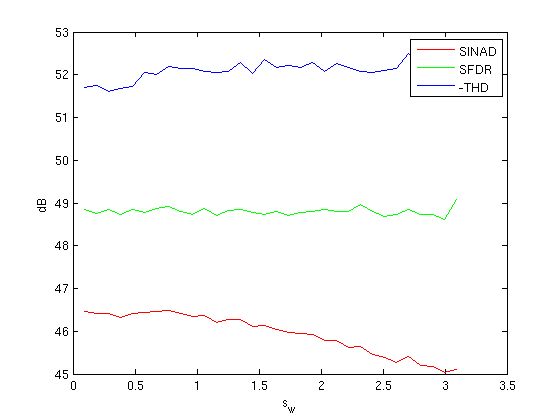
\includegraphics[width=\textwidth]{./pics/snrplots.png}
 % snrplots.png: 560x420 pixel, 90dpi, 15.81x11.85 cm, bb=0 0 448 336
 \caption{Plot of the different performance measures, SINAD, SFDR and THD over normalized frequency s\_W}
 \label{fig:snrplots}
\end{figure}


\begin{figure}[h!]
 \centering
 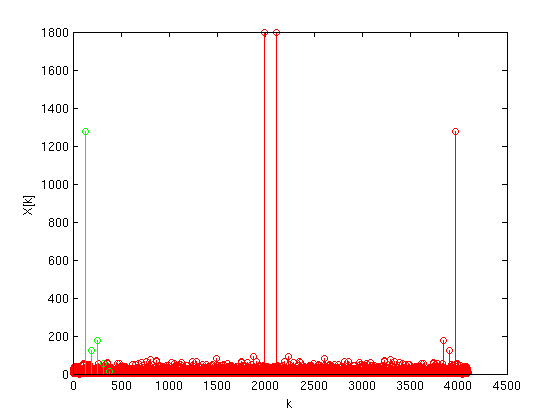
\includegraphics[width=\textwidth]{./pics/spectrum.png}
 % snrplots.png: 560x420 pixel, 90dpi, 15.81x11.85 cm, bb=0 0 448 336
 \caption{Plot of the spectrum of the first input signal, after the signal amplitude has been
 set to 0. What you can see in the plot is the spectrum of Noise and Distortion. The
 first 5 harmonics (aliasing component of the harmonics are not displayed in green) are marked as green.}
 \label{fig:spectrum}
\end{figure}







\end{document}